\documentclass{article}
\usepackage[slovak]{babel}
\usepackage[left=2cm,right=2cm]{geometry}
\usepackage{graphicx}
\usepackage{hyperref}
\usepackage[table]{xcolor}
\newcolumntype{a}{p{2cm}}
\newcolumntype{b}{p{2cm}}
\definecolor{g}{HTML}{EEDDEE}
\definecolor{r}{HTML}{DDEEEE}

\begin{document}
\begin{center}
\vskip 1cm
\Huge
\textbf{Laboratórny protokol}\\
\medskip
\LARGE
Meranie hustoty objektov\\
\medskip
\textbf{Adam Jenča}\\
\medskip
\large
Príma A\\
\medskip
Fyzika
\vskip  3cm
\tableofcontents
\end{center}
\newpage
\large
\section{Teoretický Úvod}
Hustota $\varrho_x$ popisuje pomer hmotnosti a objemu  kocky vyrobenej z materiálu $x$.\\
Vzorec pre hustotu pri hmotnosti $m$ a objeme $V$ je $\varrho = \frac{m}{V}$.
\subsection{Jednotky hustoty}
Jednotky hustoty sa píšu vo formáte $\frac{J_m}{J_V}$ kde $J_m$ je jednotka hmotnosti a $J_V$ je jednotka objemu.\\
Základná jednotka hustoty je $\frac{g}{cm^3}$ ($\varrho_x = n\frac{g}{cm^3}$ znamená, že kocka z materiálu $x$ s objemom $1\ cm^3$ váži $n$ gramov) .
\section{Popis experimentu}
\begin{figure}[h]
    \centering
    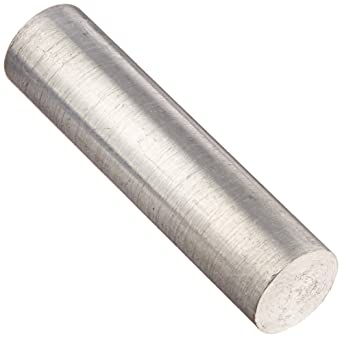
\includegraphics[width=0.25\textwidth]{al.jpg}
    \label{fig:valec}

    \caption{Valček z neznámeho materiálu(hliníka)}
    \end{figure}
Potrebujeme zistiť hustotu neznámeho materiálu a porovnať ju s jeho tabuľkovou hustotou. Máme k dispozícii 4 valčeky z tohto materiálu (pozri \textbf{Obrázok 1}), každý inej veľkosti.
\subsection{Pomôcky}
Na experiment potrebujeme:
\begin{itemize}
 \item  odmerný valec
 \item  váhy
 \item  valčeky z neznámeho materiálu
 \item  vodu
\end{itemize}
\subsection{Postup}
\begin {enumerate}
\item  Pre každý valček:
\begin{enumerate}
\item   Pomocou váh odmeriame hmotnosť valčeka $m_n$
\item   Odmeriame objem valčeka $V_n$ nasledovne:
\begin{enumerate}
\item    Do odmerného valca napustíme dostatočné množstvo vody
\item    Odmeriame objem vody vo valci $V_n^1$
\item    Vložíme valček do vody tak, aby bol úplne ponorený
\item    Odmeriame objem vody vo valci po vložení valčeka $V_n^2$
\item    Vypočítame objem valčeka pomocou vzorca $V_n=V_n^2-V_n^1$
\end{enumerate}
\item   Vypočítame hustotu valčeka $\varrho_n=\frac{m_n}{V_n}$
\end{enumerate}
\item  Vypočítame priemernú hustotu 
	$  \overline{ \varrho}$ pomocou vzorca 
	\[
		\overline{ \varrho}=\frac{ \displaystyle \sum _{n=1} ^{ 4} \varrho_n}{4}=\frac{ \varrho_1+\varrho_2+\cdots+\varrho_4}{ 4}.
	\] 
\item Porovnáme $ \overline{ \varrho}$ s tabuľkovou hustotou $\varrho_{TAB}$
\end{enumerate}
\section{Výpočty}
\subsection{Tabuľka}
\begin{center}
\begin{tabular}{  p{1cm}  p{2cm}  p{2cm}  p{2cm}  p{2cm}  p{2cm} }
	\rowcolor{r}
	Valček & $V_n^1$ & $V_n^2$ & $V_n$ & $m_n$ & $\varrho_n$ \\
	\rowcolor{g} 
	$1$ & $41.1 cm^3$ & $45.3 cm^3$ & $4.2 cm^3$ & $13.3 g$ & $3.1\overline{6} \frac{g}{cm^3}$ \\
	\rowcolor{r}
	$2$ & $41.7 cm^3$ & $48.3 cm^3$ & $6.6 cm^3$ & $18.8 g$ & $2.\overline{84} \frac{g}{cm^3}$ \\
	\rowcolor{g}
	$3$ & $30.2 cm^3$ & $43.3 cm^3$ & $13.1 cm^3$ & $27.2 g$ & $2.07633 \frac{g}{cm^3}$ \\
	\rowcolor{r}
	$4$ & $80.1 cm^3$ & $99.3 cm^3$ & $19.2 cm^3$ & $38.2 g$ & $1.99 \frac{g}{cm^3}$ \\
	
\end{tabular}
\end{center}
\subsection{Valček 1}
\begin{enumerate}
	\item Vypočítame $V_1$:
	\[
		V_1=45.3 cm^3-41.1cm^3=4.2cm^3
	\]
	\item Vypočítame $\varrho_1$:
	\[
		\varrho_1 = \frac{m_1}{V_1} = \frac{13.3}{4.2} = 3.1\overline{6} \frac{g}{cm^3}
	\]

	\end{enumerate}
\subsection{Valček 2}
	\begin{enumerate}
	\item Vypočítame $V_2$:
	\[
		V_2=48.3 cm^3-41.7cm^3=6.6cm^3
	\]
	\item Vypočítame $\varrho_2$:
	\[
		\varrho_2 = \frac{m_2}{V_2} = \frac{18.8}{6.6} = 2.\overline{84} \frac{g}{cm^3}
	\]

	\end{enumerate}
\subsection{Valček 3}
	\begin{enumerate}
	\item Vypočítame $V_3$:
	\[
		V_3=43.3 cm^3-30.2cm^3=13.1cm^3
	\]
	\item Vypočítame $\varrho_3$:
	\[
		\varrho_3 = \frac{m_3}{V_3} = \frac{27.2}{13.1} = 2.07633 \frac{g}{cm^3}
	\]

	\end{enumerate}
\subsection{Valček 4}
\label{sec:v4}
	\begin{enumerate}
	\item Vypočítame $V_4$:
	\[
		V_4= 99.3 cm^3-80.1cm^3=19.2cm^3
	\]
	\item Vypočítame $\varrho_4$:
	\[
		\varrho_4 = \frac{m_4}{V_4} = \frac{38.2}{19.2} = 1.99 \frac{g}{cm^3}
	\]

	\end{enumerate}
\subsection{Priemer}
	\[
		\overline{ \varrho}=\frac{\varrho_1+\varrho_2+\varrho_3+\varrho_4}{4} = \frac{3.1\overline{6}+2.\overline{84}+2.07633+1.99}{4} = 2.52037037\frac{g}{cm^3}
	\]
\newpage
\section{Porovnanie}
Tabuľková hustota $\varrho_{TAB} = 2.70 \frac{g}{cm^3}$.\\
Priemerná hustota $\overline{\varrho} =  2.52037037 \frac{g}{cm^3}$.\\
Rozdiel hustôt $\varrho_d = abs(\varrho_{TAB}-\overline{\varrho}) =  0.17962963  \frac{g}{cm^3} $\\
\section{Záver}
Výsledok vyšiel dosť presne, s rozdielom menším ako $0.2 \frac{g}{cm^3}$.\\
Rozdiel $0.2 \frac{g}{cm^3}$ vznikol pravdepodobne pri \hyperref[sec:v4]{štvrtom meraní}, \\
keďže tam vyšla výrazne nižšia hustota ako $\varrho_{TAB}$ ($1.99 \frac{g}{cm^3}$) \\
Pravdepodobne som sa pomýlil pri meraní objemu $V_4$, lebo je pri ňom väčšia chyba merania ako pri hmotnosti $m_4$.\\
Táto chyba mohla vzniknúť tým. že som sa do odmerného valca nepozeral kolmo, ale šikmo zvrchu.
Oveľa presnejšie výsledky ako pri meraní objemu ponáraním do kvapaliny v odmernom valci sa dajú dosiahnuť vypočítaním objemu valca:
\[
	V_c=(\pi \times r_c^2)\times v_c,
\]
kde $r_c$ je polomer a $v_c$ je výška valca $c$.
\end{document}
